\documentclass[a4paper]{ltjsarticle}
\usepackage{color}
\usepackage{comment}
\usepackage[bottom=25mm]{geometry} % 余白等の設定
\usepackage{lastpage} % 最後のページ番号を \pageref{LastPage} で取得
\usepackage{fancyhdr} % ヘッダー
\usepackage{titlesec} % Section などの設定
\usepackage[unicode]{hyperref} % PDF のメタデータ生成
\usepackage{docmute}

\usepackage{amsfonts} % 整数全体の集合とかの記号を表すフォント
\usepackage{bm}       % 数式でベクトルを表す太字斜体
\usepackage{braket}   % Dirac の Braket 記法

\usepackage[version=4]{mhchem}   % 化学式
\usepackage{chemfig}  % 構造式
\usepackage{siunitx}  % SI unit
\usepackage{listing}  % コード

\makeatletter

% maketitle
\@addtoreset{section}{part}
\titleformat{\part}{\centering\Large}{}{0em}{}
\titlespacing{\part}{0pt}{0ex}{1cm}
\newcommand{\repotitle}[1]{\def\@repotitle{#1}}
\newcommand{\gakuseinumber}[1]{\def\@gakuseinumber{#1}}
\renewcommand{\maketitle}{
    % 表紙にするときはコメントアウト
    \thispagestyle{empty}
    \pagenumbering{gobble}
    \vspace*{\stretch{1}}
    \begin{center}
        \vspace*{0.4cm}
        {\Huge{\@title}}
        \vspace{1cm}

        {\Large \@date}

        \vspace{0.5cm}

        {\Large \@gakuseinumber \quad \@author}

        \vspace{1cm}
    \end{center}
    \vspace{\stretch{1}}
    \newpage
    \pagenumbering{arabic}
}


% Header
\pagestyle{fancy}
\lhead{\@repotitle \qquad \@gakuseinumber \quad \@author}
\rhead{Page \thepage\ of \pageref{LastPage}}
\fancyfoot{}
\fancypagestyle{nofooter}
\makeatother

% Macros
\newcommand{\uL}[0]{\si{\micro L}}
\newcommand{\ug}[0]{\si{\micro g}}

%%%% Title %%%%%%%%%%%%%%%%%%%%%%%%%%%%%%%%%%%%%%%%%%%%%%%%%%%%%%%%%%%%%%%%%%%%%
\repotitle{分析化学実験 5 レポート}
\title{分析化学実験 5 レポート \\ \vspace{1.5ex} {\LARGE --- 生化学分析 ---}}
\author{宗形 翼}
\gakuseinumber{03-200796}
\date{\today}
\hypersetup{
    pdftitle={分析化学実験 5 レポート},
    pdfauthor={宗形 翼}
}

\begin{document}

\part{実験B タンパク質のイオン交換分離とゲル電気泳動による確認}

% ____
% |  _ \ _   _ _ __ _ __   ___  ___  ___
% | |_) | | | | '__| '_ \ / _ \/ __|/ _ \
% |  __/| |_| | |  | |_) | (_) \__ \  __/
% |_|    \__,_|_|  | .__/ \___/|___/\___|
%                  |_|
\section{目的}

タンパク質をイオン交換分離し、
SDS ポリアクリルアミドゲル電気泳動によってを定性する。


%  _____                      _                      _
% | ____|_  ___ __   ___ _ __(_)_ __ ___   ___ _ __ | |_
% |  _| \ \/ / '_ \ / _ \ '__| | '_ ` _ \ / _ \ '_ \| __|
% | |___ >  <| |_) |  __/ |  | | | | | | |  __/ | | | |_
% |_____/_/\_\ .__/ \___|_|  |_|_| |_| |_|\___|_| |_|\__|
%            |_|
\section{実験}



\subsection{器具}

\begin{itemize}
    \item 電気泳動装置(BIO-RAD)
    \item 水平回転振蕩器
    \item イオン交換筒
    \item バット
\end{itemize}

\subsection{試薬}

\begin{itemize}
    \item 陰イオン交換樹脂(BIO-RAD)
    \item 緩衝液 (A 液) : 10 mM Tris/HCl pH 8.2
    \item 緩衝液 (B 液) : 10 mM Tris/HCl pH 8.2 containing 500 mM NaCl
    \item サンプル Buffer : 試験管に 0.5 M Tris/HCl (pH 6.8) 1 mL、0.1 \% BPB 0.5 mL、10 \%
        SDS 1.6 mL、グリセリン 0.8 mL、2-メルカプトエタノール 0.4 mL と水 4 mL を加え混合する。
    \item 泳動用緩衝液 : 25 mM Tris, 192 mM Glycine, 0.1\%SDS 溶液とし HCl にて pH 8.3 に 調整する。
    \item 泳動用ゲル (READY GELS J、分離ゲル 4-20\%T、 BIO-RAD)
    \item 分子量マーカー (250~10 kDa、BIO-RAD)
    \item CBB溶液 (タンパク質染色用色素 CoomassieBrilliantBlue)
    \item 各種タンパク質 (以下のタンパクの内、等電点が離れている3種を選択する)
\end{itemize}


\subsection{操作}

混合タンパク質に A 液 2mL を加えて、スターラーを用いてゆっくり溶解させ、
混合タンパク質溶液を作成する。混合タンパク質溶液 100 \uL に A 液 900 \uL を加えて
1/10 混合タンパク質溶液とする。

クロマト管にイオン交換樹脂 5mL を加え、下部からの水滴の滴下が無くなったら
押さえフィルターを手フロン棒を使用して挿入する。
これに A 液を約 50 mL 流して洗浄したのちキャップを閉める。

10mL 目盛り付き試験管7つに、A 駅と B 駅をそれぞれ以下の体積比で混合し
分取用溶液を調製する。\\
A 液 : B 液 \quad 10 : 0 \quad 9 : 1 \quad 8 : 2 \quad 7 : 3 \quad
6 : 4 \quad 5 : 5 \quad 4 : 6

イオン交換カラムに混合タンパク質溶液を 1.5 mL 添加し、溶出液は廃棄する。
水滴の滴下が無くなったら分取用溶液を \ce{NaCl} 濃度が低い順、
つまり B 液の割合が小さい順に滴下し溶出駅を採取し、
同じ順番で UV スペクトルを計測する。

8本の 1.5 mL マイクロチューブに、50 \si{\micro L} サンプル Buffer と
1/10 混合タンパク質溶液を 50 \uL をそれぞれ加え、
マイクロチューブホルダーをつけ熱湯に3分間浸漬する。
放冷したのちホルダーを外して泳動用資料とする。

泳動層に泳動用ゲルを装填したのち、
泳動用緩衝液を注入し漏れがないことを確認する。
その後外側にも緩衝液を入れる。

1 mL マイクロピペッターを用いてウェルを緩衝液で洗浄後、
20 \uL ピペッターを用いてウェルに泳動用資料を 5 \uL 注入し、
150 V の定電圧で電気分解を行い、気泡が生じることを確認する。
30分から40分後、青色が泳動層先端まで来ていることを確認し
定電圧装置の電源を切る。

泳動層からゲルを外し、破らないように注意しながら CBB 溶液に浸し、
水平回転振盪器で約1時間激しく揺らす。
ゲルを水に移し水平回転振盪器で1時間洗浄し、撮影する。

%  ____                 _ _
% |  _ \ ___  ___ _   _| | |_
% | |_) / _ \/ __| | | | | __|
% |  _ <  __/\__ \ |_| | | |_
% |_| \_\___||___/\__,_|_|\__|
\section{結果}

UV スペクトルから 280nm ピークの吸光度を読み取り図 \ref{fig:uv} に示した。

図 \ref{fig:result} から複数のタンパク質が含まれていることがわかるので、
分離は不完全であったことがわかるが、
A液とB液の体積比が6:4においてはコンアルブミンのみシグナルが出ており、
コンアルプミンのみ単離できたことがわかる。

分離ゲルの上端から角栄同バンドの中心までの距離の比を
\ref{fig:result} から計測し、表 \ref{table:kyori} に示した。

先に求めた泳動距離を最も短いものを1とする相対距離に変換し、
それをx軸に、y軸に分子量をプロットした(図 \ref{fig:kenryo})。
最小二乗法で検量線を作成する際に、
とりえる全ての相対移動度の区間で $ R^2 $ 値を求めたところ、
相対移動度が最も小さい 3 つを除いた区間が
$ R^2 = 0.986 $ で最大だったので、
その区間の値のみを用いて検量線を作成した。

その検量線から分子量が 71, 29, 15 kDa と定量できた。
そこからコンアルプミン、カルボニックアンヒトラーぜ、
ミオグロビンと同定できた。

% ____  _                        _
% |  _ \(_)___  ___ _   _ ___ ___(_) ___  _ __
% | | | | / __|/ __| | | / __/ __| |/ _ \| '_ \
% | |_| | \__ \ (__| |_| \__ \__ \ | (_) | | | |
% |____/|_|___/\___|\__,_|___/___/_|\___/|_| |_|
\section{考察}

図 \ref{fig:result} の No.1, No.2 の間でミオグロビン、
カルボニックアンヒドラーゼが無くなっているので
A液とB液の割合を10:0から9:1の間で細かく区切れば、
ミオグロビンとカルボにクアンヒドラーぜを分離できると考えられる。

%  ____            _     _
% |  _ \ _ __ ___ | |__ | | ___ _ __ ___
% | |_) | '__/ _ \| '_ \| |/ _ \ '_ ` _ \
% |  __/| | | (_) | |_) | |  __/ | | | | |
% |_|   |_|  \___/|_.__/|_|\___|_| |_| |_|
\section{設問}

\subsection{(1)}

緩衝液の pH は8.2だからタンパク質は不の電荷を帯びているので、
pI が大きいタンパク質ほど早く溶出すると考えられる。

\subsection{(2)}

ベンゼン環を持つフェニルアラニン、トリプトファン、チロシン
(図 \ref{fig:amino})が考えられる。

\begin{figure}[!hbtp]
\minipage{0.32\textwidth}
\chemfig[atom sep=2em]{
H_2N-[:30](-[:90]-[:30]*6(-=-=-=))-[:-30](=[:-90]O)-[:30]OH
}
\endminipage\hfill
\minipage{0.32\textwidth}
\chemfig[atom sep=2em]{
H_2N-[:30](-[:90]-[:30]*5(=-NH-(*6(-=-=-=))--))-[:-30](=[:-90]O)-[:30]OH
}
\endminipage\hfill
\minipage{0.32\textwidth}
\chemfig[atom sep=2em]{
H_2N-[:30](-[:90]-[:30]*6(-=-(-OH)=-=))-[:-30](=[:-90]O)-[:30]OH
}
\endminipage
\centering\caption{フェニルアラニン、トリプトファン、チロシン}
\label{fig:amino}
\end{figure}

\subsection{(3)}

設問1で述べたようにタンパク質は不電荷を帯びているので
下部電極は陽極である。

\subsection{(4)}

サンプルの比重をバッファと近くする役割。

\subsection{(5)}

タンパク質の \ce{S-S} 結合を切断し、立体構造を破壊する役割。



% _____ _
% |  ___(_) __ _ _   _ _ __ ___  ___
% | |_  | |/ _` | | | | '__/ _ \/ __|
% |  _| | | (_| | |_| | | |  __/\__ \
% |_|   |_|\__, |\__,_|_|  \___||___/
%          |___/
\begin{figure}[p]
    \begin{center}
        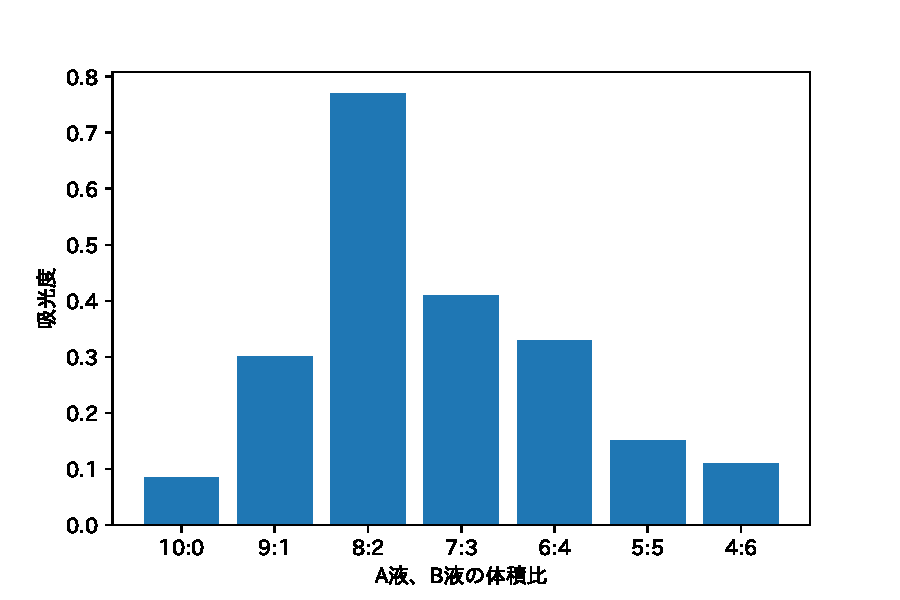
\includegraphics[width=0.8\textwidth]{1.pdf}
        \caption{UV スペクトルの 280 \si{nm} の吸光度}
        \label{fig:uv}
    \end{center}
\end{figure}

\begin{figure}[p]
    \begin{center}
        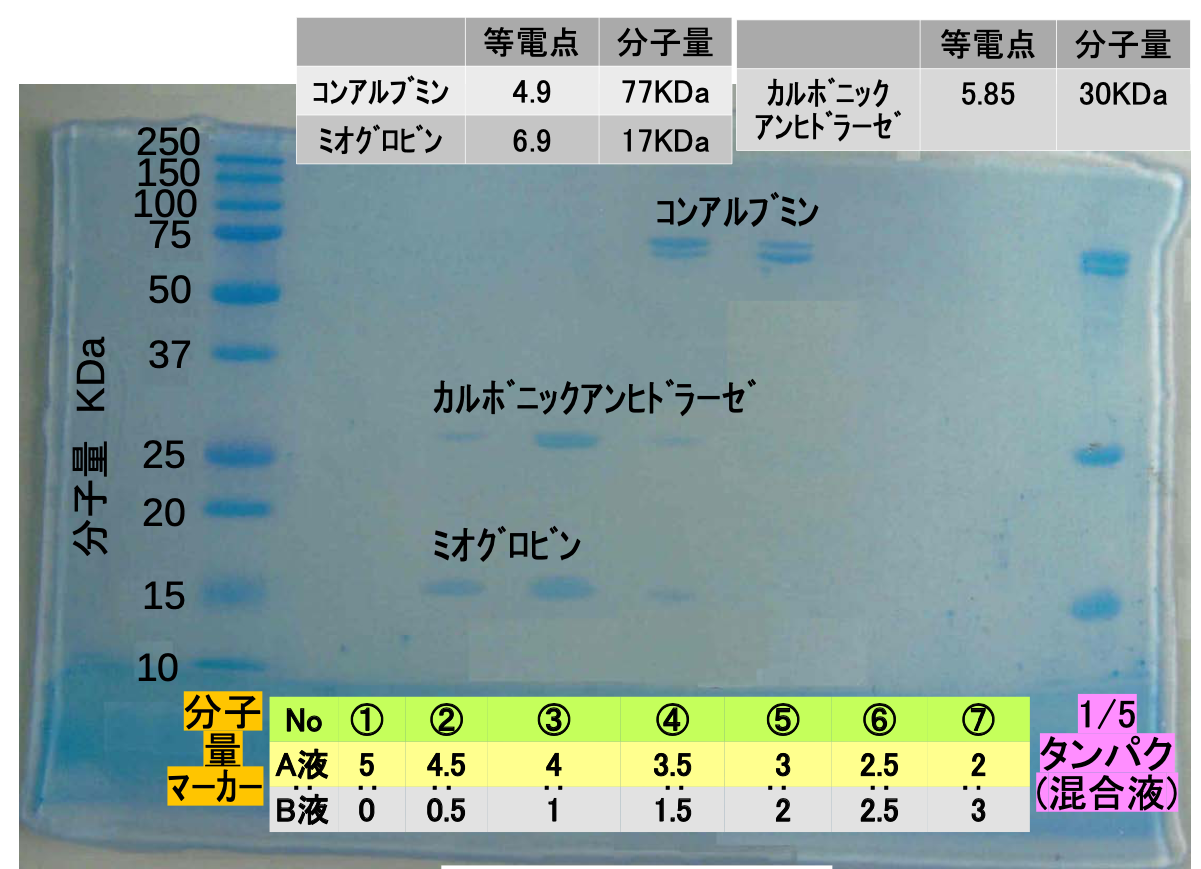
\includegraphics[width=0.8\textwidth]{result.png}
        \caption{分子量マーカーの電気泳動結果}
        \label{fig:result}
    \end{center}
\end{figure}

\begin{table}[p]
    \centering
    \caption{電気泳動でのタンパク質の移動距離}
    \label{table:kyori}
    \begin{tabular}{cc}
        \hline
        分子量 kDa & 泳動距離 [px] \\
        \hline
        250 & 22 \\
        150 & 41 \\
        100 & 67 \\
        75 & 95 \\
        50 & 155 \\
        37 & 215 \\
        25 & 318 \\
        20 & 372 \\
        15 & 457 \\
        10 & 526 \\
        \hline
    \end{tabular}
\end{table}

\begin{figure}[p]
    \begin{center}
        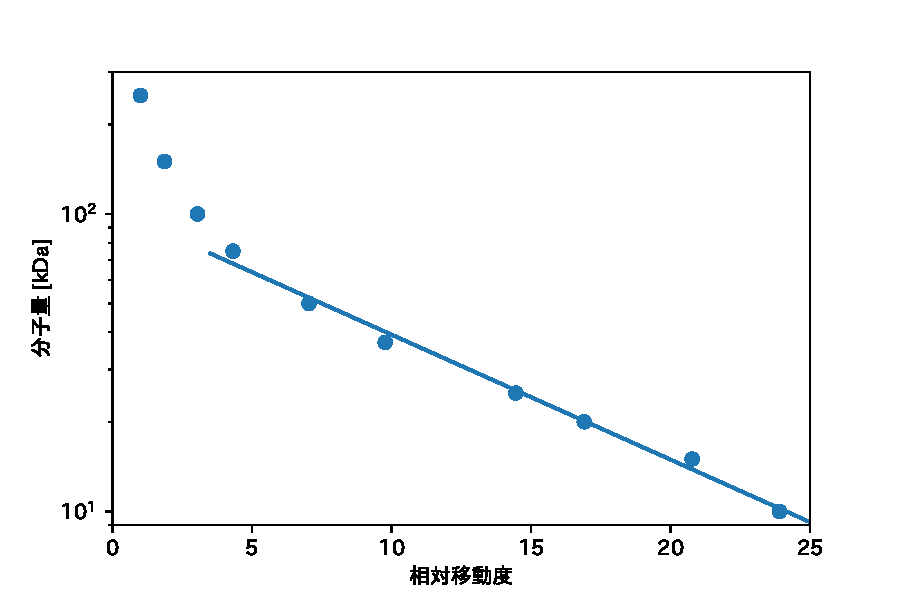
\includegraphics[width=0.8\textwidth]{kenryo.pdf}
        \caption{電気泳動の結果}
        \label{fig:kenryo}
    \end{center}
\end{figure}

\end{document}
